\documentclass[conference]{IEEEtran}

\usepackage{amssymb,amsmath}
\usepackage{wrapfig}
\usepackage{multirow}
\usepackage{graphicx}
\usepackage{algorithm}
\usepackage{algorithmic}
\usepackage{times}
\usepackage{cite}
\usepackage{url}
\usepackage{booktabs}
\usepackage{subfigure}
\usepackage{fancybox}
\usepackage{color}
\usepackage{array}
\usepackage{subfigure}
\usepackage{balance}
\usepackage{epstopdf}
\usepackage{array}
\usepackage[normalem]{ulem}
\usepackage{csquotes}

\newcommand{\everton}[1]{\textcolor{yellow}{{\it [Everton: #1]}}}
\newcommand{\emad}[1]{\textcolor{red}{{\it [Emad: #1]}}}
\newcommand{\todo}[1]{\colorbox{yellow}{\textbf{[#1]}}}

\newcommand{\conclusionbox}[1]{%
	\vspace{2mm}
	\framebox[0.45\textwidth][c]{%
		\parbox[b]{0.42\textwidth}{%
			{\it #1}
		}
	}
	\vspace{2mm}
}

\newcommand{\rqi}{\textbf{RQ1- What are the types of self-admitted technical debt found in code comments? How they are distributed across different software projects?}}

\begin{document}
\title{A Taxonomy of Self-Admitted Technical Debt Types}

\author{\IEEEauthorblockN{Everton da S. Maldonado and Emad Shihab}

\IEEEauthorblockA{Department of Computer Science and Software Engineering\\Concordia University,
Montreal, Canada\\
\url{e_silvam@encs.concordia.ca}, \url{emad.shihab@concordia.ca}}}

\maketitle

\begin{abstract} Technical Debt is a term that has been used to express non-optimal solutions during the development of software projects. These non optimal solutions are often shortcuts that allow the project to move faster in the short term, at the cost of increased maintenance in the future. To help alleviate the impact of technical debt, a number of studies focused on the detection of technical debt. More recently, our work should that one possible source to detect technical debt is using source code comments, also referred to as self-admitted technical debt. However, what types of technical debt can be detected using source code comments remains as an open question.
	
Therefore, in this paper we explore the examine code comments to determine the different types of technical debt. First, we propose four simple filtering heuristics to eliminate comments that are not likely to contain technical debt. Second, we read through more than 33K comments, and we find that self-admitted technical debt can be classified into five main types - design debt, defect debt, documentation debt, requirement debt and test debt. The  most common type of self-admitted technical debt is design debt, making up between 42\% to 84\% of the classified comments. Lastly, we make the classified dataset of more than 33K comments publicly available for the community as a way to encourage future research and the evolution of the technical debt landscape.
%We also find that of all classified comments 7.42\% represent some type of technical debt
	
\end{abstract}

\IEEEpeerreviewmaketitle

\section{Introduction}
\label{sec:introduction}
The software development process is filled with challenges. There are short deadlines, complex changes that need to be made, high quality expectations and an ever changing environment. Often there is much more that needs to be done than time to accomplish it. This puts developers under increasing pressure to implement their tasks, while achieving many conflicting constraints. In this context, some decisions are made to allow the short term development of the project at the cost of its increased maintenance effort in the future. This phenomena is know as Technical Debt \cite{Cunningham1992}. 

With the organization of the technical debt community through the managing technical debt workshop \cite{Falessi2014MTD}, recent work has focused on the detection of technical debt \cite{Potdar2014ICSME} \cite{Zazworka2013CSE}, studying the impact of technical debt \cite{Zazworka2011MTD}
and the appearance of technical debt in the form of code smells \cite{Fontana2012MTD}. Despite many efforts to detect technical debt, its detection remains a challenge~\cite{Potdar2014ICSME}. One relatively unexplored aspect of technical debt is self-admitted technical debt, that is technical debt reported in source code comments. Self-admitted technical debt refers to the situation where developers know that the current implementation is not optimal and write comments alerting the inadequacy of the solution. 

Recently, Potdar and Shihab~\cite{Potdar2014ICSME} developed an approach to identify technical debt from code comments, and through manual inspection, were able to mine 62 patterns that effectively identify self-admitted technical debt. However, their approach does not take into consideration the different types of technical debt. Understanding the different types of self-admitted technical debt is important since: 1) it helps the community understand the limitations of understanding technical debt through code comments, 2) it allows us to complement existing technical debt detection approaches and 3) it provides us with a better understanding of the developer's point of view of technical debt.

Therefore, in this paper we examine and quantify the different types of self-admitted technical debt. To do so, we extract source code comments from 5 well commented open source projects that belongs to different application domains, namely Apache Ant, Apache Jmeter, ArgoUml, Columba and JFreeChart. In total, we examined more than 166K comments. We applied a set of 4 simple filtering heuristics to remove comments that are not likely to contain self-admitted technical debt (e.g., license comments, commented source code, Javadoc comments). Finally, these filtering heuristics resulted in a dataset of 33,093 comments that the first author manually analyzed and classified into different types of self-admitted technical debt.

When classifying the code comments, we found 5 types of self-admitted technical debt which are: design debt, defect debt, documentation debt, requirement debt and test debt. Analyzing the distribution of the comments we found that the most common type of self-admitted technical debt is design debt, making up between 42\% - 84\% of all the classified comments. In addition to our findings, we contribute a rich dataset of self-admitted technical making the data used in this study publicly available. To the best of our knowledge, there is not similar data available and we believe that the dataset will encourage future research in the area of self-admitted technical providing the necessary foundation for more advanced techniques as Natural Language Processing.  

The rest of the paper is organized as follows. Section \ref{sec:related_work} presents related work. We describe our approach and setup our case study in Section \ref{sec:approach}. Section \ref{sec:results} presents the case study results. The threats to validity are presented in Section \ref{sec:threats_to_validity} and in Section \ref{sec:conclusion} concludes the paper and discusses future work. 

\section{Related Work}
\label{sec:related_work}

\subsection{Comment related work}

Other work used code comments to understand developer tasks. For example. Storey \textit{et al.}~\cite{Storey2008ICSE} analyzed how task annotations (e.g., TODO, FIXME) play a role in improving team articulation and communication. The work closest to ours is the work by Potdar and Shihab~\cite{Potdar2014ICSME}, where code comments were used to identify technical debt. 

Similar to some of the prior work. we also use source code comments to identify technical debt. However, our main focus is on the detection of . As we have shown, our approach yield different and better results in detection . Furthermore, we propose comment patterns, that are derived from source code comments, to detect .

\subsection{Technical debt related work}

A number of studies have focused on the study of, detection and management of technical debt. Much of this work has been driven by the Managing Technical Debt Workshop effort. Fore example, Seaman \textit{et al.}~\cite{Seaman2011}, Kruchten \textit{et al.}~\cite{Kruchten2013IWMTD} and Brown \textit{et al.}~\cite{Brown2010MTD} make several reflections about the term technical debt and how it has been used to communicate the issues that developers find in the code in a way that managers can understand. Alves \textit{et al.} \cite{Alves2014MTD} complement this work by proposing a ontology on technical debt terms. Given the fact that this is a recent research area with publication dating only since 2010. In their work they gathered definitions and indicators of technical debt that was scattered across the literature, and as a result their ontology provides several different types of technical debt (e.g., architecture debt, build debt, code debt, design debt, defect debt, etc) grouped by their nature (i.e., the factor that lead to the introduction of the debt at the first place).  

Other work focused on the detection of technical debt. Zazworka \textit{et al.} \cite{Zazworka2013CSE} conducted an experiment to compare the efficiency of automated tools in comparison with human elicitation regarding the detection of technical debt. They found that there is small overlap between the two approaches, and thus it is better to combine them than replace one with the other. In addition, they concluded that automated tools are more efficient in finding defect debt, whereas developers can realize more abstract categories of technical debt.

In follow on work, Zazworka \textit{et al.}~\cite{Zazworka2011MTD} conducted a study to measure the impact of technical debt on software quality. They focused on a particular kind of design debt, namely God Classes. They found that God Classes are more likely to change, and therefore, have a higher impact in software quality. Fontana \textit{et al.}~\cite{Fontana2012MTD} investigated design technical debt appearing in the form of code smells. They used metrics to find three different code smells, namely God Classes, Data Classes and Duplicated Code. They proposed an approach to classify which one of the different code smells should be addressed first, based on a risk scale. Also related here, Potdar and Shihab~\cite{Potdar2014ICSME} used code comments to detect technical debt.They extracted the comments of four projects and analyzed more than 101,762 comments to come up with 62  patterns that indicates self-admitted technical debt. Their findings show that 2.4\% - 31\% of the files in a project contain self-admitted technical debt.

%Our work is different from the work that uses code smells to detect design technical debt since we use code comments to detect design technical debt. Also, our focus is on \emph{self-admitted} design technical debt. As we have shown in the discussion section, there is very little overlap between the  that our approach detects and the design technical debt detected using code smells (in particular God classes)

%The above work provide the necessary background to complement previous work of potdar.

\todo{add comparison between works and prune it better}

\section{Approach}
\label{sec:approach}
\begin{figure*}[thb!]
  \centering
  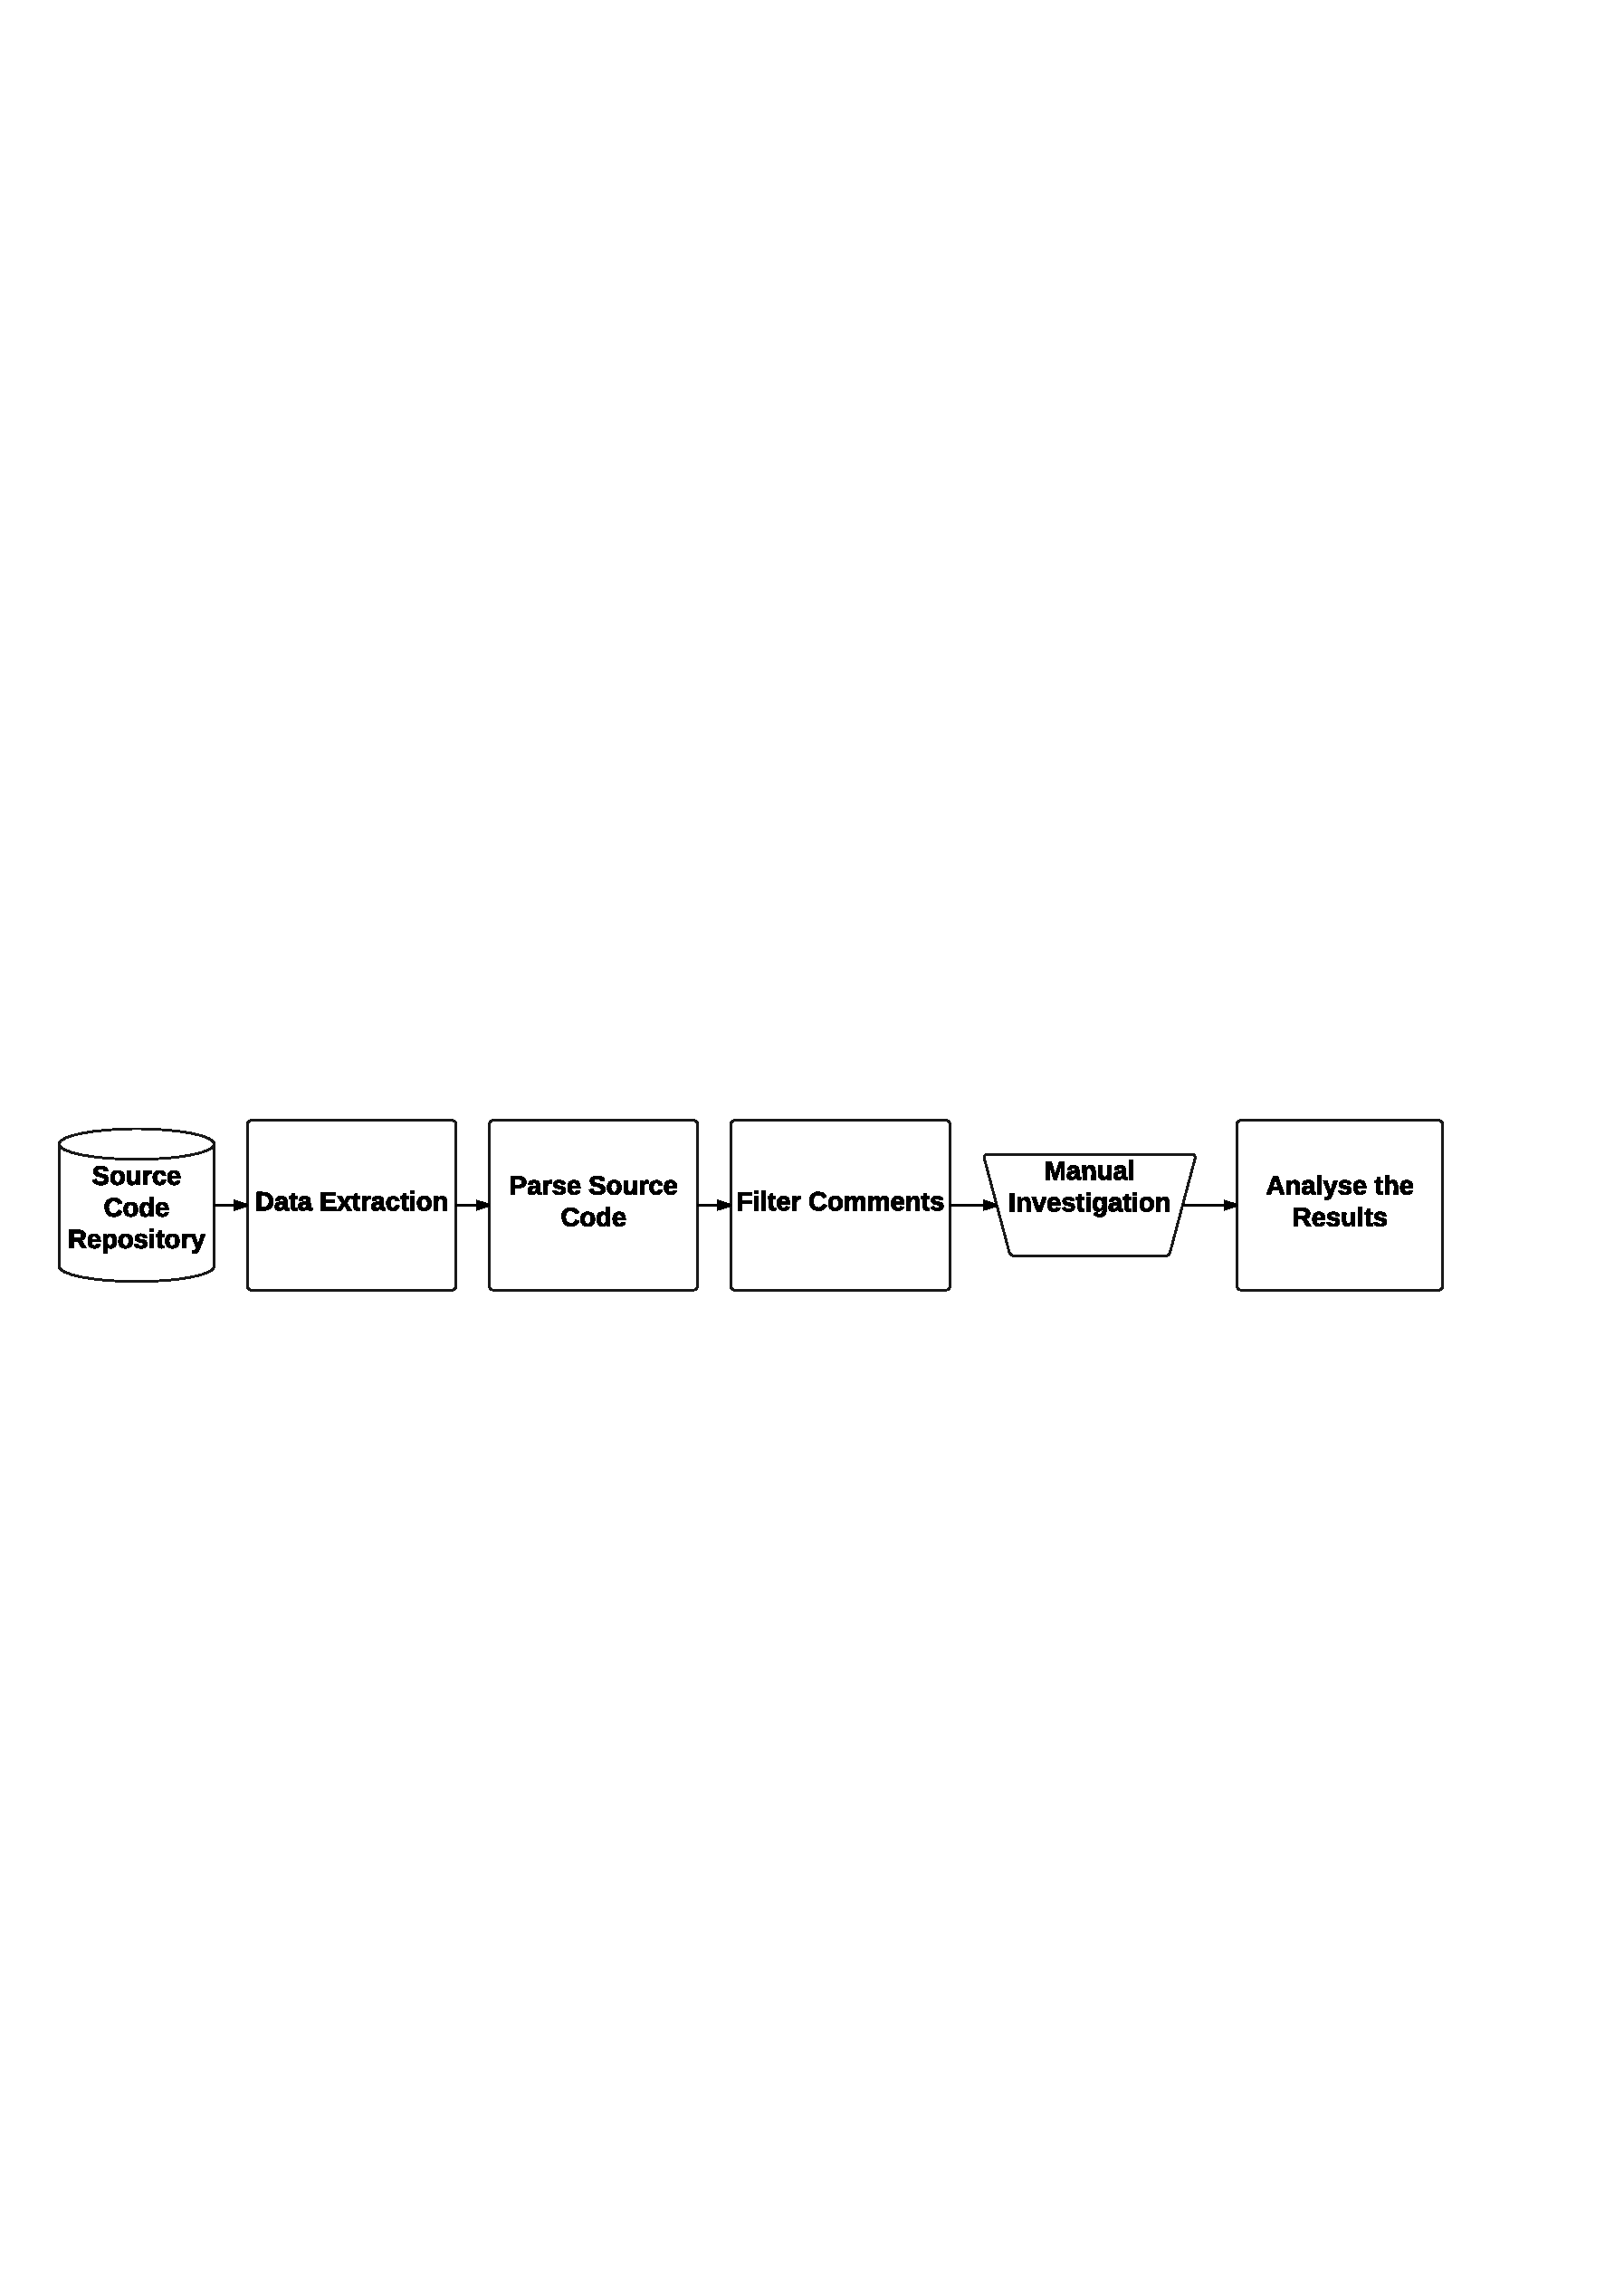
\includegraphics[width=1\textwidth]{figures/Approach}
  \caption{Approach overview}
  \label{fig:approach}
\end{figure*}

\begin{table*}[!hbt]
      \begin{center}
            \caption{Project Details}
            \label{tab:project_details}
            \begin{tabular}{l| c c r c c }
            \toprule
            \textbf{Project}   & \textbf{Release}  & \textbf{\# of classes}   & \textbf{SLOC}    & \textbf{\# of comments}  & \textbf{\# of contributors} \\ \midrule 
              Apache Ant       & 1.7.0             &  1,475                   & 115,881          & 21,587                   & 74  \\                       
              Apache Jmeter    & 2.10              &  1,181                   &  81,307          & 20,084                   & 33  \\                         
              ArgoUML          & 0.34              &  2,609                   & 176,839          & 67,716                   & 87  \\               
              Columba          & 1.4               &  1,711                   & 100,200          & 33,895                   & 9   \\                   
              JFreeChart       & 1.0.19            &  1,065                   & 132,296          & 23,474                   & 19  \\ \bottomrule
            \end{tabular}
      \end{center}
\end{table*}

The main goal of our study is to identify and quantify the different types of self-admitted technical debt found in source code comments. Figure \ref{fig:approach} shows an overview of our approach, and the following subsections detail each step of it.

\subsection{Project Data Extraction} % (fold)
\label{sub:project_data_extraction}

To perform our study, we obtain the source code of five open source projects, namely Apache Ant, Apache Jmeter, ArgoUML, Columba and JFreeChart. We chose the aforementioned projects, since they belong to different application domains, and vary in size (e.g., SLOC), and in the number of contributors.

Table \ref{tab:project_details} provides statistics about each one of the projects used in our study. We provide details about the release used, the number of classes, the total source lines of code (SLOC), the total extracted comments and the number of contributors. A source line of code contain at least one valid character, which is not blank spaces or source code comments. In our study, we only use the Java files to calculate the SLOC, and to do so, we use the tool SLOCCount \cite{wheeler2004:home}. 

The number of contributors was extracted from OpenHub, an on-line community and public directory that offers analytics, search services and tools for open source software \cite{Openhub:home}. It is important to notice that the number of comments shown for each project does not represent the number of commented lines, but rather the number of individual line, block, and Javadoc comments. In total, we obtained more than 166,756 comments, found in 8,041 Java classes.
% subsection data_extraction (end)
 
\subsection{Parse Source Code} % (fold)
\label{sub:parse_source_code}

After obtaining the source code of all projects, we extract the comments from their source code. We use JDeodorant \cite{Tsantalis2008CSMR}, an open-source Eclipse plug-in, to parse the source code and extract the code comments. JDeodorant is capable of identify design flaws (i.e., bad smells) in Java projects, and suggest refactoring opportunities to solve them. JDeodrant uses the Eclipse AST framework to create an Abstract Syntax Tree (AST) map of the source code. The AST map contains detailed information about the project such as: the source code comments, its type (i.e., Block, Single-line or Javadoc), the line where each one of these comments begins and finishes. We extract the aforementioned information and store all comments in a relational database to facilitate the processing of the data.

% subsection parse_source_code (end) 

\subsection{Filter Comments} % (fold)
\label{sub:filter_comments}

Source code comments can be used for different purposes in a project like giving context, as part of the documentation, to express thoughts, opinions and authorship, and in some cases, to remove source code from the program. Comments are used freely for developers and with few formalities, if any at all. This informal environment allows developers to bring to light opinions, insights and even confessions (e.g., self-admitted technical debt). 

As shown in prior work by Potdar and Shihab \cite{Potdar2014ICSME}, part of these comments can be identified as self-admitted technical debt, but they are not the majority of cases. With that in mind, we develop and apply 4 filtering heuristics to narrow down the comments eliminating the ones that are less likely to be classified as self-admitted technical debt.

To do so, we developed a Java based tool that reads from the database the data obtained by parsing the source code. Next, it executes the filtering heuristics and stores the result back in the database. The retrieved data contains information like the line number that a class/comment begins/ends and the type, considering the Java syntax, of the comment (i.e., Block, Single-line or Javadoc). With this information we process the filtering heuristics as described next.

We found that license comments are very not likely to contain self-admitted technical debt, and that license comments are commonly added before the declaration of the class. Therefore, we create a heuristic that removes comments that are placed before the class declaration. Since we know the line number that the class was declared we can easily check for comments that are placed before that line and remove them. In order to decrease the chances of removing a self-admitted technical debt comment while executing this filter we calibrated this heuristic to not remove comments containing one of task-reserved words (i.e., ``todo'', ``fixme'', or ``xxx'').

We also notice that some times developers make long comments, using multiple \emph{single-line} comments instead of a Block comment. This characteristic can hinder the understanding of the message. Consider the case that the reader (i.e., human or machine) analyze each one of these comments independently, the message would be incomplete and the meaning lost. To solve that problem, we create a heuristic that searches for consecutive single-line comments and groups them as one. We identify consecutive comments by subtracting the line number of both comments. If the result of the difference is equals a -1 we have a consecutive comment. For example, Single-line comment A is placed in line number 100 and Single-line comment B is placed in line 101. The subtraction of the line numbers will result in -1, therefore the comments are consecutive.
 
Similarly, is common to find commented source code across the projects, and this can be due to many different reasons. One of the possibilities is that the code is not being used, other is that the code is used for debug purposes only. Based on our analysis, commented source code does not have self-admitted technical debt. Our heuristic remove commented source code using a simple regular expression that captures typical Java code structures.

% else\s*\{|try\s\{|do\s*\{|finally\s*\{|if\s*\(|for\s*\(|while\s*\(|switch\s*\(|Long\s*\(|Byte\s*\(|Double\s*\(|Float\s*\(|Integer\s*\(|Short\s*\(|BigDecimal\s*\(|BigInteger\s*\(|Character\s*\(|Boolean\s*\(|String\s*\(|assert\s*\(|System.out.|public\s*void|private\s*static*final|catch\s*\( 

Lastly, when analyzing Javadoc comments we found that they rarely mention self-admitted technical debt. For the Javadoc comments that does mention self-admitted technical debt we notice that they usually contains one of the task-reserved words (i.e., ``todo'', ``fixme'', or ``xxx''). Based on this, our heuristic remove all comments of the type Javadoc unless they contain at least one of the task-reserved words. To do so, we create a simple regular expression that search for the task-reserved words before removing the comment.  

The steps mentioned above significantly reduced the number of comments in our dataset and helped us focus on the most applicable and insightful comments. For example, in the Apache Ant project, applying the above steps helped reduce the number of comments from 21,587 to 4,140 comments meaning that 19.17\% of the comments were kept for analysis. Table \ref{tab:filtering_heuristics_details} provides details for each one of the projects.

\begin{table}[!hbt]
      \begin{center}
            \caption{Filtering heuristics details}
            \label{tab:filtering_heuristics_details}
            \begin{tabular}{l| p{0.55in} p{0.75in} p{0.75in} }
            \toprule
            \thead{\textbf{Project}}   & \textbf{Total \# of comments}  & \textbf{\# of comments after filtering} & \textbf{\%  of TD-related comments}\\ \midrule 
              Apache Ant       & 21,587                & 4,140                   & 19.17 \% \\ 
              Apache Jmeter    & 20,084                & 8,163                   & 40.64 \% \\
              ArgoUML          & 67,716                & 9,788                   & 14.45 \% \\              
              Columba          & 33,895                & 6,569                   & 19.38 \% \\
              JFreeChart       & 23,474                & 4,436                   & 18.89 \% \\ \bottomrule
            \end{tabular}
      \end{center}
\end{table}
% subsection filter_comments (end)

\subsection{Manual Classification} % (fold)
\label{sub:manual_classification}

To classify the comments, we developed a Java based tool that shows one comment at a time and gives a list of possible classifications that can be manually assigned to the comment. The list of possible classifications is based on previous work by Alves \textit{et al.}~\cite{Alves2014MTD}. After applying the different filtering steps, we successfully classified 33,093 comments. The more than 33 thousand comments were classified into five different types of self-admitted technical debt, i.e., design debt, defect debt, documentation debt, requirement debt and test debt.

The first author who made the classification has more than 8 years of experience working in the industry as a software engineer, during this time he designed, implemented and maintained several programs using, in particular the Java programming language. He developed solid skills in object orientated programming and design patterns. We consider that these qualifications provide the necessary background to conduct the manual classification of the comments.   
% subsection manual_classification (end)


\section{Case Study Results}
\label{sec:results}
The goal of our study is to classify and quantify the different types of self-admitted technical debt. To do so, we divide our study in two parts first, we manually read trough all comments identifying self-admitted technical debt among them. Once identified, the self-admitted technical debt, is classified into different types. Second, we quantify these comments identifying the most common types. Our case study is formalized with the following research question:


%In the remainder of this section we detail the motivation, approach and results for our research question. 

\vspace{3mm}
\noindent\rqi
\vspace{3mm}

\noindent\textbf{Motivation:} As shown in previous work \cite{Potdar2014ICSME}, self-admitted technical can be an indicator of non-optimal solutions. However, technical debt is a general term, and there are many different types of technical debt \cite{Alves2014MTD}. Although we know that self-admitted technical exists, the different types of self-admitted technical debt are still unknown. For example, are we able to detect documentation debt from code comments? Answering this question is important as different types of debt have different approaches to be solved, and therefore each different type may need a tailored solution. It also helps us understand the opportunities and limitations of using code comments to detect technical debt. 

\vspace{1mm}
\noindent\textbf{Approach:} To identify the different types of debt found in the comments we manually read through source code comments as described in Section \ref{sec:approach}. While examining the comments we classify each comment by the nature of the debt, using the descriptions provided by Alves \textit{et al.} as a guideline. 

During the classification we notice that some comments can be classified in more than one type of debt (e.g., a comment reporting a design debt can also be causing an unexpected behavior, which is defect debt). Although this is an ambiguous situation, and may have different interpretations depending of who is reading the comments, we defined that each comment would have just one classification type for the sake of clarity. To mitigate the chance of misclassifying these comments, we take in consideration the more meaningful type for each comment in a given scenario. To do so, whenever a case like this occurred, we did a more detailed investigation (i.e., by examining the source code and any available documentation). In total we read and classified 33,093 comments from five open source projects. The classification took approximately 95 hours and was performed by the first author of the paper. 

\vspace{1mm}
\noindent\textbf{Results:} We found five different types of self-admitted technical debt. Below, we list the different types of technical debt that we were able to detect and provide example comments to help the reader grasp the different types of self-admitted technical debt comments.


\begin{itemize}
  \item \textbf{Self-admitted design debt:} These comments indicate that there is a problem with the design of the code. They can be comments about misplaced code, lack of abstraction, long methods, poor implementation, workarounds or a temporary solution. Lets consider the following comments:
  
  \vspace{1mm}
  \begin{displayquote}
     \textit{``TODO: - This method is too complex, lets break it up''}
     
     \vspace{1mm}

     \textit{``/* TODO: really should be a separate class */''}
  \end{displayquote}
  \vspace{1mm}

These comments are clear examples of what we consider as self-admitted \emph{design debt}. In the above comments, the developers state what needs to be done in order to improve the current design of the code. Although the above comments are easy to understand, during our study we came across more challenging comments that expressed design problems in an indirect way. For example: 
  
  \vspace{1mm}
  \begin{displayquote}
     \textit{``// I hate this so much even before I start writing it. // Re-initialising a global in a place where no-one will see it just // feels wrong.  Oh well, here goes.''}

     \vspace{1mm}

     \textit{``//quick \& dirty, to make nested mapped p-sets work:''}
  \end{displayquote}
  \vspace{1mm}

In the above example comments the authors are certain to be implementing code that does not represent the best solution. Intuitively, we know that kind of implementation will degrade the design of the code and should be avoided. 

  \vspace{1mm}
  \begin{displayquote}
      \textit{``// probably not the best choice, but it solves the problem of // relative paths in CLASSPATH''}

      \vspace{1mm}

      \textit{``//I can't get my head around this; is encoding treatment needed here?''}
  \end{displayquote}
  \vspace{1mm}

The above comments expressed doubt and uncertainty when implementing the code and were considered as self-admitted design debt as well.

\item \textbf{Self-admitted defect debt:} In defect debt comments the author states that a part of the code does not have the expected behavior, meaning that there is a defect in the code. 
  
  \vspace{1mm}
  \begin{displayquote}
      \textit{``// Bug in above method''}

      \vspace{1mm}

      \textit{``// WARNING: the OutputStream version of this doesn't work!''}
  \end{displayquote}
  \vspace{1mm}
  
As shown in these examples there are defects that are known by the developers, but for some reason is not fixed yet. 

  \item \textbf{Self-admitted documentation debt:} In the documentation debt comments the author express that there is no proper documentation supporting that part of the program.
  
  \vspace{1mm}
  \begin{displayquote}
  	\textit{``**FIXME** This function needs documentation''}
  	
  	\vspace{1mm}
  	
  	\textit{``// TODO Document the reason for this''}
  \end{displayquote}
  \vspace{1mm}
  
  Here, the developers clearly recognize the need to document their code, however, for some reason they do not document it yet.
  
  \item \textbf{Self-admitted requirement debt:} Requirement debt comments express incompleteness of the method, class or program as observed in the following comments:
  
  \begin{displayquote}
  	\textit{``/TODO no methods yet for getClassname''}
  	
  	\vspace{1mm}
  	
  	\textit{``//TODO no method for newInstance using a reverse-classloader''}

  	\vspace{1mm}
  	
  	\textit{``TODO: The copy function is not yet * completely implemented - so we will  * have some exceptions here and there.*/''}  
  	
  \end{displayquote}
  \vspace{1mm}  
  
The last example shows a comment that could be considered as having more than one type of debt. (i.e., requirement debt and defect debt), but as mentioned in the classification approach, we choose to maintain one type only for each comment. 
  	
Based on our understanding, the defect debt expressed in the comment would not exist if the requirement debt did not exists. Therefore, the main debt in this comment is a requirement debt (i.e., incomplete implementation of the copy function). 
  	
%One more reason that we give a comment only one classification type is that there is no way to tell if the other requirement debts are not causing an unexpected behavior, except in the case that the author of the comment express is. 
  
  \vspace{1mm}
  \item \textbf{Self-admitted test debt:} Test debt comments are the ones that express the need for implementation or improvement of the current tests. As shown in the examples below, test debt comments are very straight forward in their meaning. 
  
  \begin{displayquote}
  	\textit{``// TODO - need a lot more tests''}
  	
  	\vspace{1mm}
  	
  	\textit{``//TODO enable some proper tests!!''}
  \end{displayquote}
  \vspace{1mm}  
    
\end{itemize}

After classifying the comments, we notice that not all of the types mentioned in by Alves \emph{et al.}~\cite{Alves2014MTD} could be found. We argue that some types like people debt or infrastructure debt are less probable to appear in source code comments. Other types such as build debt could not be found because we are examining comments in Java classes only, not taking in consideration build scripts that are usually written in other languages (e.g., Maven and Ant use XML files as build scripts). 

%Other than that, types like test automation debt and test debt were considered as self-admitted test debt in our study due to the resemblance of their purpose. In a similar way, process debt, service debt, code debt and architecture debt were considered as self-admitted design debt in our study.

\conclusionbox{We find five different types of self-admitted technical debt, i.e., design debt, defect debt, documentation debt, requirement debt and test debt.}
%Although there are comments that can have more the one type of debt, we found that there is a main type of debt that the comment can be classified to.

\begin{figure*}[thb!]
  \centering
  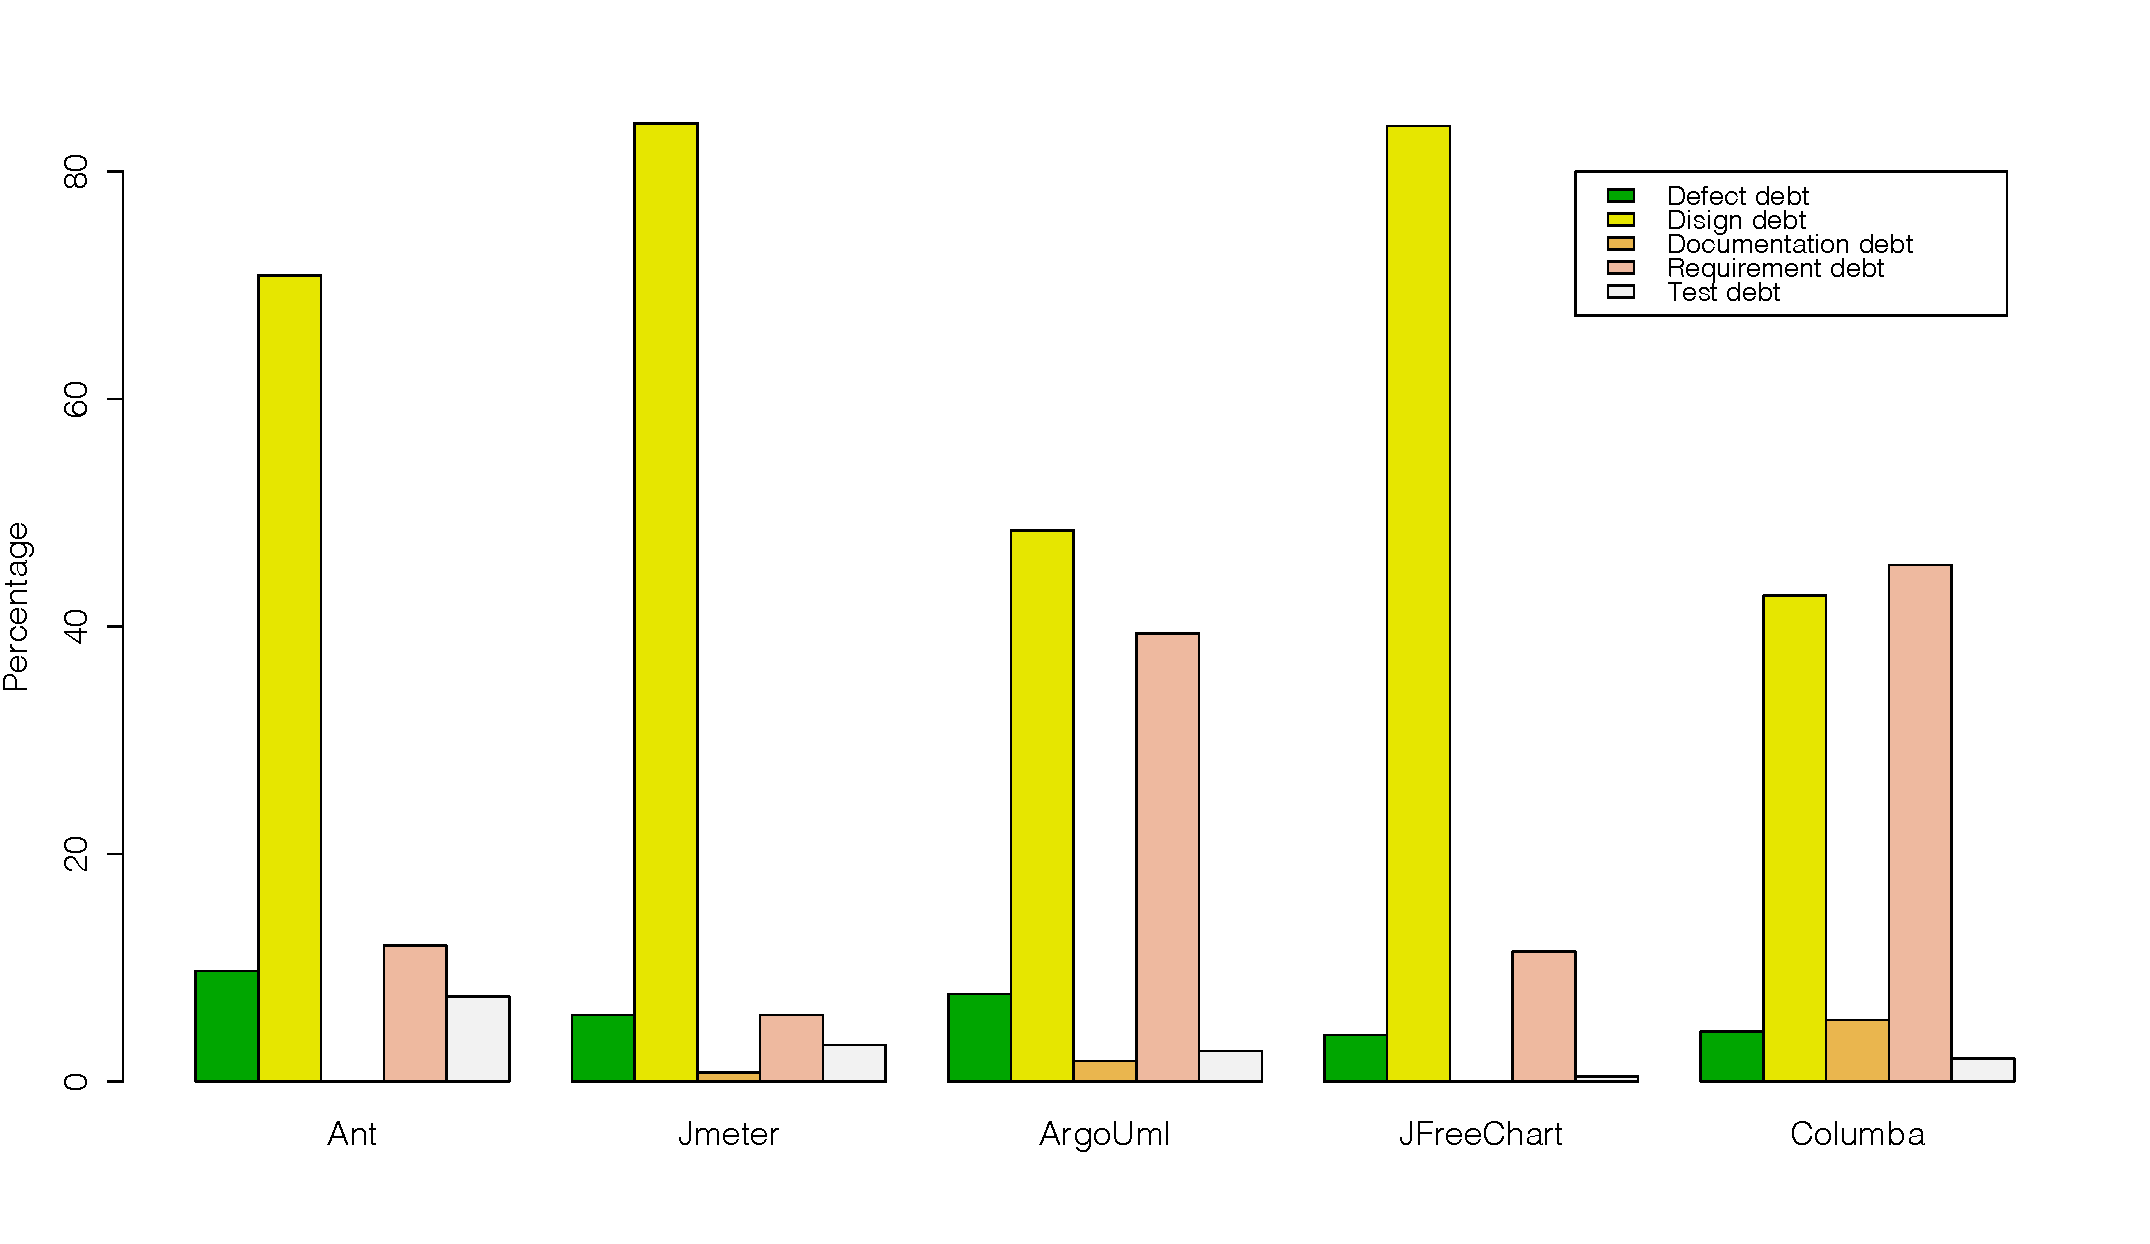
\includegraphics[width=1\textwidth]{figures/technical_debt_distribution.pdf}
  \caption{Self-admitted technical debt types distribution}
  \label{fig:satd_distribution}
\end{figure*}

In addition to determining the different type of self-admitted technical debt, we would like to quantify the different types. Doing so will help us understand the strengths and weaknesses of using code comments to detect technical debt. After analyzing the more than 33K comments, we found that only 2,457 comments are self-admitted technical debt comments, representing 7.42\% (i.e., $\frac{2457}{33093}$) of all the classified comments. The percentage of self-admitted technical debt found for each project is presented in Table~\ref{tab:total_self_admitted_per_project}. ArgoUml is the project with the highest percentage of self-admitted technical debt and Apache Ant has the lowest percentage, amounting to 16.8\% and 3.2\% respectively.

\begin{table}[!hbt]
     \begin{center}
           \caption{Self-admitted technical debt per project}
           \label{tab:total_self_admitted_per_project}
           \begin{tabular}{l| c c c }
           \toprule
           \textbf{Project}      & \textbf{\# comments}     & \textbf{\# self-admitted TD} & \textbf{\%} \\ \midrule 
             Apache Ant          & 4,140                          & 134                                & 3.2  \\                                   
             Apache Jmeter       & 8,163                          & 375                                & 4.6  \\                                   
             ArgoUML             & 9,788                          & 1,653                              & 16.8 \\                                   
             Columba             & 6,569                          & 295                                & 4.4 \\                                   
             JFreeChart          & 4,433                          & 219                                & 4.9  \\ \bottomrule
           \end{tabular}
     \end{center}
\end{table}

Figure \ref{fig:satd_distribution} shows the percentage of each type of self-admitted technical debt across the projects. Since each project has a different number of comments we normalized the data, presenting the percentages of the different types rather than the raw numbers. For example, if a project has 100 self-admitted technical debt comments and 10 where design debt type, we say that the project has 10\% of self-admitted design technical debt. 

Analyzing the Figure \ref{fig:satd_distribution} we find that self-admitted design debt is the most common in 4 out of 5 projects. Self-admitted design technical debt values ranged from 42\%, in Columba project with the lowest percentage, to 84\% in Jmeter and JFreeChart, projects with the highest percentage. The second most frequent type is self-admitted requirement debt with values between 5\% and 45\%, followed by self-admitted defect technical debt making up between 4\% to 9\% of the comments. Self-admitted test technical debt ranged from 0\% to 7\% whereas self-admitted documentation debt had only 0\% to 5\% of the comments.     

We notice that Columba and ArgoUml have the highest occurrences of self-admitted requirement debt. Columba is a email client application written in Java, which has 9 contributors \cite{Openhub:home}, and a considerable number of classes 1,711. It is reasonable to think that developers have limited time to develop features. Therefore, leaving comments of features that need to be implemented in the future (i.e., requirement debt) is more likely. 

%Another aspect to consider is the domain of the project, that way developers do not need to necessarily wait for the next requirement to know what need to be implemented, although time still a constraint. Based on these observations, we assume that the hight number of self-admitted requirement technical debt in Columba reflects that the project has not reached yet its full potential regarding to features. 

ArgoUml has a hight number of contributors 87 and yet has a hight number of self-admitted requirement debt. We argue that the domain and complexity of the application may explain these numbers. As an UML modeling tool, ArgoUml itself is impacted for external changes like different implementations of UML language (e.g., 1.2 , 1.3 and then 1.4) trough every change there may be many features that need to be refactored. \emad{try to look for a stronger argument here.}

%For the other projects we assume that they reach a maturity point where all the main features was implemented and the majority of the problems are related to the design of the code. 

\conclusionbox{We find that the majority of the self-admitted technical debt comments are design debt, which ranged from 42\% to 84\% across the projects. The second most frequent type was requirement debt that ranged from 5\% to 45\%. The remaining types have low frequency if considered that they represented less than 10\% of the occurrences}

\section{Threats to validity}
\label{sec:threats_to_validity}
\noindent\textbf{Internal validity} consider the relationship between theory and observation, in case the measured variables do not measure the actual factors. To classify the source code comments we heavily depended on manual classification due the fact that comments are written in natural language and therefore needed to be interpreted by a human. Like any human activity, our manual classification is subject to personal bias and subjectivity. To reduce this bias in the future we will ask to other researchers of our lab to classify the dataset, verifying and discussing possible divergences of opinion. Changes in this dataset may impact our findings. When performing our study, we used well-commented Java projects. Since our technique heavily depends on code comments, our results and performance measures may be impacted by the quantity and quality of comments in a software project.  

\noindent \textbf{External validity} consider the generalization of our findings. All of our findings were derived from comments in open source projects. To minimize external validity, we chose open source projects from different domains. That said, our results may not generalize to other open source or commercial projects. In particular, our results may not generalize to projects that have a low number or no comments. Other than that, we only analyze projects written in Java, the results obtained may not generalize to projects written in other languages.

\section{Conclusion and Future work}
\label{sec:conclusion}
The term technical debt is being used for practitioners and researchers in the software engineer community to express shortcuts and workarounds employed in software projects. These shortcuts will most often impact the maintainability of the project hindering the development if not addressed properly.

Our work explore specifically self-admitted technical debt, that is the technical debt deliberately introduced by the developers and reported by the same trough source code comments.

In our study we analyzed the comments of 5 open source projects which are Apache Ant, Apache Jmeter, ArgoUml , Columba and JFreeChart. These projects are considered well commented and they belong to different application domains. We used them to understand the characteristics of self-admitted technical debt types creating a rich dataset with more than 33,093 classified comments.

In our approach we present 4 simple filtering heuristics that made feasible the hard task to manually classify the comments of a project. These filtering heuristics significantly reduced the number of comments filtering approximately 81\% of the 166,756 extracted comments. This allowed the classification to be focused on the most applicable and insightful comments which was 33,093 comments in total. 

We find that self-admitted technical debt can be classified into the following types: design debt, defect debt, documentation debt, requirement debt and test debt. We also provide concrete examples of each one of the mentioned types and the rationale to classify them as it was.  

We also find that the majority of the self-admitted technical debt comments are of the design debt type. It ranged from 42\% to 84\% across the projects. The second most frequent type was requirement debt that ranged from 5\% to 45\%. Based on this result, we can say that the self-admitted technical debt types that developers cares the most are related with the design of the program and implementation of future features, outranking documentation and test debt.

Other contribution of our study is that we make publicly available the resulting dataset of our classification. We hope that this will encourage future research in the area of self-admitted technical debt as, to the best of our knowledge, this is the first dataset of this kind. We also think that the information provided by this dataset can be a cornerstone for more advanced techniques as natural language processing.   

In a future work we plan to improve the current classification adding more projects to it. With a richer dataset we expect that more patterns and characteristics of the self-admitted technical types will be retrieved. We also plan to use this database to mine unique sequential patterns, an advanced technique of natural language processing which may lead to innovative ways to identify self-admitted technical debt. 


\bibliographystyle{IEEEtran}
\balance
\bibliography{bib}

\end{document}
